% Template created by Karol Kozioł (www.karol-koziol.net) for ShareLaTeX

\documentclass[a4paper,9pt]{extarticle}
\usepackage[utf8]{inputenc}
\usepackage[T1]{fontenc}
\usepackage{graphicx}
\usepackage{xcolor}
\usepackage{tikz}
\usepackage{fontawesome}
\usepackage{hyperref}
\hypersetup{
    colorlinks=true,
    linkcolor=blue,
    filecolor=magenta,      
    urlcolor=blue,
}
 
\urlstyle{same}

\usepackage{amsmath,amssymb,textcomp}
\everymath{\displaystyle}

\usepackage{times}
\renewcommand\familydefault{\sfdefault}
\usepackage{tgheros}
\usepackage[defaultmono,scale=0.85]{droidmono}

\usepackage{multicol}
\setlength{\columnseprule}{0pt}
\setlength{\columnsep}{20.0pt}

% Style for coding: Starts %
\usepackage{listings}
\usepackage{color}

\definecolor{dkgreen}{rgb}{0,0.6,0}
\definecolor{gray}{rgb}{0.5,0.5,0.5}
\definecolor{mauve}{rgb}{0.58,0,0.82}

\lstset{frame=tb,
  language=Python,
  aboveskip=3mm,
  belowskip=3mm,
  showstringspaces=false,
  columns=flexible,
  basicstyle={\small\ttfamily},
  numbers=none,
  numberstyle=\tiny\color{gray},
  keywordstyle=\color{blue},
  commentstyle=\color{dkgreen},
  stringstyle=\color{mauve},
  breaklines=true,
  breakatwhitespace=true,
  tabsize=3
}

% Style for coding: Ends %

\usepackage{geometry}
\geometry{
a4paper,
total={210mm,297mm},
left=10mm,right=10mm,top=10mm,bottom=15mm}

\linespread{1.3}

% custom title
\makeatletter
\renewcommand*{\maketitle}{%
\noindent
\begin{minipage}{0.65\textwidth}

\begin{tikzpicture}
\node[rectangle,rounded corners=6pt,inner sep=10pt,fill=blue!50!black,text width= 0.95\textwidth] {\color{white}\Huge \@title};
\end{tikzpicture}
\end{minipage}
\hfill
\begin{minipage}{0.25\textwidth}
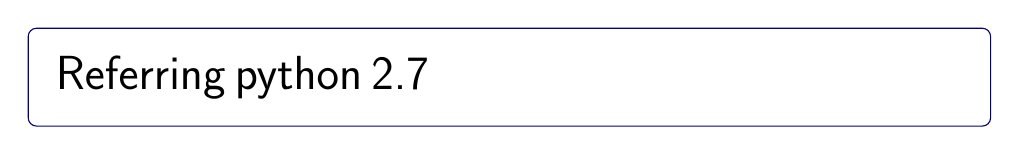
\begin{tikzpicture}
\node[rectangle,rounded corners=3pt,inner sep=10pt,draw=blue!50!black,text width= 0.95\textwidth] {\LARGE Referring python 2.7};
\end{tikzpicture}
\end{minipage}
\bigskip\bigskip
}%
\makeatother

% custom section
\usepackage[explicit]{titlesec}
\newcommand*\sectionlabel{}
\titleformat{\section}
  {\gdef\sectionlabel{}
   \normalfont\sffamily\Large\bfseries\scshape}
  {\gdef\sectionlabel{\thesection\ }}{0pt}
  {
\noindent
\begin{tikzpicture}
\node[rectangle,rounded corners=3pt,inner sep=4pt,fill=blue!50!black,text width= 0.95\columnwidth] {\color{white}\sectionlabel#1};
\end{tikzpicture}
  }
\titlespacing*{\section}{0pt}{15pt}{10pt}


% custom footer
\usepackage{fancyhdr}
\makeatletter
\pagestyle{fancy}
\fancyhead{}
\fancyfoot[C]{\footnotesize \textcopyright\ \@date\ \ \@author}
\renewcommand{\headrulewidth}{0pt}
\renewcommand{\footrulewidth}{0pt}
\makeatother

\title{Python for JAVA Developers: Basics V 1.1}
\author{Akash Panchal - www.medium.com/@akashp1712}
\date{2018}

\begin{document}

\maketitle
\begin{multicols*}{2}

\section{Basic Syntax}
\subsection{End of Statements}
Unlike the Java, to end a statement in Python, we don't have to type in a semicolon, you simply press \boxed{Enter}. But semicolons can be used to delimit statements if you wish to put multiple statements on the same line.
\begin{lstlisting}
message1 = 'Hello World!'
message2 = "Python gives no missing semicolon error!"

# Instead of System.out.print, we use print
print message1 # print 'Hello World!' on the console output
print "Hello"; print "Python!";  # usage of the semicolon

\end{lstlisting}

\subsection{Code Blocks and Indentation}
One of the most distinctive features of Python is its use of indentation to mark blocks of code.
Consider the following if-statement from our non-zero number checking program:

\textbf{JAVA}
\begin{lstlisting}
if (0 == value) {
    System.out.print("Number is Zero");
} else {
    System.out.print("Number is non-Zero.");
}

System.out.print("All done!");
\end{lstlisting}

\textbf{Python}
\begin{lstlisting}
if 0 == value:
    print('Number is Zero')
else:
    print('Number is non-Zero.')

print('All done!')
\end{lstlisting}

To indicate a block of code in Python, you must indent each line of the block by the same amount. The two blocks of code in our example if-statement are both indented \textbf{four spaces}, which is a typical amount of indentation for Python.

\section{Variables}

\subsection{Declaration}
Variables are created the first time a value is assigned to them. There is no concept of the declaration of the data type in python.
\begin{lstlisting}
number = 11
string = "This is a string"
\end{lstlisting}
You declare multiple variables by separating each variable name with a comma.
\begin{lstlisting}
a, b = True, False
\end{lstlisting}

\subsection{Assigning Values}
\begin{lstlisting}
a = 300
\end{lstlisting}
The same value can be assigned to multiple variables at the same time:
\begin{lstlisting}
a = b = c = 1
\end{lstlisting}
And multiple variables can be assigned different values on a single line:
\begin{lstlisting}
a, b, c = 1, 2, "john"
\end{lstlisting}
This is the same as:
\begin{lstlisting}
a = 1
b = 2
c = "john"
\end{lstlisting}

\section{Data Types}
Python sets the variable type based on the value that is assigned to it. Unlike JAVA, Python will change the variable type if the variable value is set to another value.

\begin{lstlisting}
var = 123 # This will create a number integer assignment
var = 'john' # the `var` variable is now a string type.
\end{lstlisting}

\subsection{Numbers}
Most of the time using the standard Python number type is fine. Python will automatically convert a number from one type to another whenever required. We don't require to use the type casting like JAVA.

\begin{center}
 \begin{tabular}{||c | c | c | c||}
 \hline
 Type & Java & Python & Description \\ [0.5ex]
 \hline\hline
 int & int a = 11 & a = 11 & Signed Integer\\
 \hline
 long & long a = 1712L & a = 1712L & (L) Long integers\\
 \hline
 float & float a = 19.91 & a = 19.91 &  (.) Floating point values\\
 \hline
 complex & - - - & a = 3.14J & (J) integer [0 to 255]\\
 \hline
\end{tabular}
\end{center}

\newpage
\subsection{String}
Create string variables by enclosing characters in quotes. Python uses single quotes \boxed{'} double quotes \boxed{"} and triple quotes \boxed{"""} to denote literal strings. Only the triple quoted strings \boxed{"""} will automatically continue across the end of line statement.

\begin{lstlisting}
firstName = 'Jane'
lastName = "Doe"
message = """This is a string that will span across multiple lines. Using newline characters and no spaces for the next lines."""
\end{lstlisting}

Key Methods:
\begin{center}
 \begin{tabular}{||c | c||}
 \hline
 Java & Python\\ [1ex]
 \hline\hline
 charAt() & find()\\
 \hline
 indexOf() & index()\\
 \hline
 length() & len()\\
 \hline
replace() & replace()\\
 \hline
 toString() & str()\\
 \hline
 trim() & rstrip(), lstrip()\\
 \hline
\end{tabular}
\end{center}

Python String comparison can be performed using equality (==) and comparison (<, >, !=, <=, >=) operators. There are no special methods to compare two strings.

\subsection{Boolean}
Python provides the boolean type that can be either set to False or True.
In python, every object has a boolean value. The following elements are false:
\begin{itemize}
  \item[$\bullet$] None
  \item[$\bullet$] False
  \item[$\bullet$] 0
  \item[$\bullet$] Empty collections: “”, (), [], {}
\end{itemize}

All other objects are True.
\textbf{Note} that, In JAVA \textbf{null} is not false while in python None is.

\subsection{List}
The List is one of the most powerful variable type (data structure!) in Python. A list can contain a series of values. Unlike JAVA, the list need not be always homogeneous. A single list can contain strings, integers, as well as objects. Lists are mutable.

List variables are declared by using brackets \boxed{[ ]} following the variable name.

\begin{lstlisting}
A = [] # This is a blank list variable.
B = [1, 23, 45, 67] # creates an initial list of 4 numbers.
C = [2, 4, 'john'] # can contain different variable types.
D = ["A", B, C] # can contains other list objects as well.
\end{lstlisting}

Key Methods:
\begin{center}
 \begin{tabular}{||c | c||}
 \hline
 Java ArrayList & Python list\\ [1ex]
 \hline\hline
 list = new ArrayList() & list=[]\\
 \hline
 list.add(object) & list.append(object)\\
 \hline
 list.get(i) & list[i]\\
 \hline
 list.size() & len(list)\\
 \hline
 list2= list.clone() & list2=list[:]\\
 \hline
\end{tabular}
\end{center}

\subsection{Tuple}
A tuple is another useful variable type similar to list and can contain heterogeneous values. Unlike the list, a tuple is \textbf{immutable} And is like a static array.

A tuple is \textbf{fixed in size} and that is why tuples are replacing array completely as they are more efficient in all parameters.

Tuple can be used as an alternative of \textbf{list(python/Java)} OR \textbf{Array(Java)} with respect to the use cases. i.e, If you have a dataset which will be assigned only once and its value should not change again, you need a tuple.

Tuple variables are declared by using parentheses \boxed{( )} following the variable name.

\begin{lstlisting}
A = () # This is a blank tuple variable.
B = (1, 23, 45, 67) # creates a tuple of 4 numbers.
C = (2, 4, 'john') # can contain different variable types.
D = ("A", B, C) # can contains other tuple objects as well.
\end{lstlisting}

\subsection{Dictionary}
Dictionaries in Python are lists of \textbf{Key: Value} pairs. This is a very powerful datatype to hold a lot of related information that can be associated through keys.
Dictionary in Python can be the Alternative of the Map in JAVA. But again a Dictionary in python can contain \textbf{heterogeneous} key as well as value.

\begin{lstlisting}
room_num = {'john': 121, 'tom': 307}
room_num['john'] = 432  # set the value associated with the 'john' key to 432
print (room_num['tom']) # print the value of the 'tom' key.
room_num['isaac'] = 345 # Add a new key 'isaac' with the associated value
print (room_num.keys()) # print out a list of keys in the dictionary
print ('isaac' in room_num) # test to see if 'issac' is in the dictionary.  This returns true.

hotel_name = {1: "Taj", "two": "Woodland", "next": 3.14} # this is totally valid in python
\end{lstlisting}

Key Methods:
\begin{center}
 \begin{tabular}{||c | c||}
 \hline
 Java HashMap & Python Dictionary\\ [1ex]
 \hline\hline
 Map myMap = new HashMap() & my\_dict = \{ \}\\
 \hline
 clear() & clear()\\
 \hline
 clone() & copy()\\
 \hline
 containsKey(key) & key \textbf{in} my\_dict\\
 \hline
 get(key) & get(key)\\
 \hline
 keySet() & keys()\\
 \hline
 put(key, value) & my\_dict[key] = value\\
 \hline
 remove(key) & pop(key)\\
 \hline
 size() & len(my\_dict)\\
 \hline
\end{tabular}
\end{center}

\section{Operators}
\subsubsection{Operator Precedence}
Operator Precedence is same as that of JAVA, let's revise it in python. Arithmetic operators are evaluated first, comparison operators are evaluated next, and logical operators are evaluated last.

\textbf{Arithmetic} operators are evaluated in the following order of precedence.

\begin{center}
 \begin{tabular}{||c | c | c||}
 \hline
 \textbf{JAVA} & \textbf{Python} & \textbf{Description}\\ [1ex]
 \hline\hline
 NOT AVAILABLE & ** & Exponentiation\\
 \hline
 - & -  & Unary negation\\
 \hline
 * & * & Multiplication\\
 \hline
 / & / & Division\\
 \hline
 \% & mod & Modulus arithmetic\\
 \hline
 + & +  & Addition\\
 \hline
 - & - & Subtraction\\
 \hline
\end{tabular}
\end{center}

\textbf{Logical} operators are evaluated in the following order of precedence.

\begin{center}
 \begin{tabular}{||c | c | c||}
 \hline
 \textbf{JAVA} & \textbf{Python} & \textbf{Description}\\ [1ex]
 \hline\hline
  ! & not & Logical negation\\
 \hline
 \&  & \& & Logical conjunction\\
 \hline
 | & | & Logical dis-junction\\
 \hline
 $\wedge$ & xor & Logical exclusion \\
 \hline
  \&\& & and & Conditional AND\\
 \hline
  || & or & Conditional OR\\
 \hline
\end{tabular}
\end{center}

\textbf{Comparison} operators all have equal precedence; that is, they are evaluated in the left-to-right order in which they appear.

\begin{center}
 \begin{tabular}{||c | c | c||}
 \hline
 \textbf{JAVA} & \textbf{Python} & \textbf{Description}\\ [1ex]
 \hline\hline
 < & < & Less than\\
 \hline
 > & > & Greater than\\
 \hline
 <= & <= & Less than or equal to \\
 \hline
  >= & >= & Greater than or equal to\\
 \hline
  == & == & Equality\\
 \hline
 != & != & Inequality\\
 \hline
 equals & is & Object equivalence \\
 \hline
\end{tabular}
\end{center}
\textbf{Note: } == in python is actually .equals() of Java.
\vspace{5 mm}

\section{Conditionals}
\subsection{if}
\begin{lstlisting}
var1 = 250
if 250 == var1:
    print "The value of the variable is 250"
\end{lstlisting}
\vspace{5 mm}

\subsection{if..else}
\begin{lstlisting}
var1 = 250
if 0 == var1:
    MyLayerColor = 'vbRed'
    MyObjectColor = 'vbBlue'
else :
    MyLayerColor = 'vbGreen'
    MyObjectColor = 'vbBlack'

print MyLayerColor
\end{lstlisting}

\subsection{if..elif..elif..else}
\begin{lstlisting}
var1 = 0
if 0 == var1:
    print "This is the first " + str(var1)
elif 1 == var1:
    print "This is the second " + str(var1)
elif 2 == var1:
    print "This is the third " + str(var1)
else:
    print "Value out of range!"
\end{lstlisting}

\subsection{Multiple conditions}
\begin{lstlisting}
skill1 = "java"
skill2 = "python"

if skill1 == "java" and skill2 == "python"
    print "Both the condition satisfy"

if skill1 == "java" or skill2 == "python"
    print "At least One condition satisfies"

\end{lstlisting}


\section{Looping}

\subsection{For Loop}
Python will automatically increments the counter (x) variable by 1 after coming to end of the execution block.
\begin{lstlisting}
for x in range(0, 5):
    print "It's a loop: " + str(x)
\end{lstlisting}

Increase or decrease the counter variable by the value you specify.
\begin{lstlisting}
# the counter variable j is incremented by 2 each time the loop repeats
for j in range(0, 10, 2):
    print "We're on loop " + str(j)

# the counter variable j is decreased by 2 each time the loop repeats
for j in range(10, 0, -2):
    print "We're on loop " + str(j)
\end{lstlisting}

You can exit any for loop before the counter reaches its end value by using the \boxed{break} statement.

\subsection{While Loop}
Simple example of while loop.
\begin{lstlisting}
var1 = 3
while var1 < 37:
    var1 = var1 * 2
    print var1
print "Exited while loop."
\end{lstlisting}
\vspace{5 mm}
Another example of while loop with break statement.
\begin{lstlisting}
while True:
    n = raw_input("Please enter 'hello':")
    if n.strip() == 'hello':
        break
\end{lstlisting}

\section{Iterations}

\subsection{Iterating a List}
\begin{lstlisting}
friends = ['Huey', 'Dewey', 'Louie']
for friend in friends:
    print 'Hello ', friend
print 'Done!'
\end{lstlisting}

\subsection{Iterating a Tuple}
\begin{lstlisting}
tup = ('alpha', 'beta', 'omega')
for val in tup:
    print val
\end{lstlisting}

\subsection{Iterating a Dictionary}
\begin{lstlisting}
codes = {'INDIA': 'in', 'USA': 'us', 'UK': 'gb'}
for key in codes:
    print key, 'corresponds to', codes[key]

# Note: key is just a variable name.
\end{lstlisting}
The above will simply loop over the keys in the dictionary, rather than the keys and values.

To loop over both key and value you can use the following:
\begin{lstlisting}
codes = {'INDIA': 'in', 'USA': 'us', 'UK': 'gb'}
for key, value in codes.iteritems():
    print key, 'corresponds to', value

# Note: key, value are just the variable names.
\end{lstlisting}

\section{The End}
That's all Folks.\newline
This ebook is made using \href{https://overleaf.com}{Overleaf}. \newline The source can be found on \href{https://github.com/akashp1712/python_cheat_sheets}{\LARGE{\faGithub}}. \newline
Thanks to \faLinkedin{} \href{https://www.linkedin.com/in/piyush-joshi-b7525216/}{Piyush Joshi} for all the guidance for this project. \newline
Visit \href{http://pythonizr.com}{Pythonizr.com} to create python boilerplate project just in \textbf{15 seconds}.

\end{multicols*}
\end{document}